\documentclass[a4paper,titlepage]{report}
\usepackage{fullpage}
\usepackage{titlesec}
\usepackage{xr}
\usepackage{array}
\usepackage{url}
\usepackage{float}
\usepackage{listings}
\usepackage{longtable}
\usepackage{enumitem}
\usepackage{graphicx}
\usepackage{verbatim}
\usepackage[dutch]{babel}
\usepackage{hyperref}
\usepackage[toc,nonumberlist,style=altlist,translate=true]{glossaries}
\usepackage{glossaries-babel}
\makeglossaries

\externaldocument[req:]{../requirements/requirements}
\externaldocument[ad:]{../architectural/architectural}

% Nummering voor subsubs en pars
\renewcommand{\thesubsubsection}{\arabic{subsubsection}}
\renewcommand{\theparagraph}{\thesubsubsection.\arabic{paragraph}}

\lstset{
    numbers=none,
    frame=shadowbox,
    identifierstyle=\ttfamily,
    keywordstyle=\color[rgb]{0,0,0},
    commentstyle=\color[rgb]{0,0,0},
    stringstyle=\color[rgb]{0,0,0},
    xleftmargin=30pt,
    xrightmargin=10pt,
    showstringspaces=false,
    breaklines=true,
    escapeinside={(*@}{@*)}
}

\makeatletter
% Label with name
\def\namedlabel#1#2{
  \label{#1}
  \begingroup
   \def\@currentlabel{#2}%
   \label{#1:name}\endgroup
}

% Reference with name
\def\namedref#1{\ref{#1} \ref{#1:name}}
\makeatother

\title{Deliverance:\\Technical Design\\Milestone 1\\Iteratie 3\\RC 3}
\author{Lucas de Vries \& Stefan van Wouw}
\begin{document}
\maketitle


% Glossary entries
\newglossaryentry{def:stuk}{name=Stuk,text=stuk,plural=stukken, description={Een
archiefstuk, boek, brochure, tijdschrift, of andere ge\"indexeerde eenheid uit
het archief of bibliotheek van het IISG. Indien een archief niet ge\"indexeerd
is, wordt het hele archief als \'e\'en stuk beschouwd. Alle stukken zijn
analoog, d.w.z. fysiek aanwezig, tenzij er wordt gesproken over digitale
stukken. Zowel de algemene metadata over een stuk, als een specifiek exemplaar
kan een `stuk' worden genoemd. Voorbeeld van onderscheid: Er zijn een aantal
exemplaren van een boek aanwezig. De contactinformatie, titel, inzage
restricties e.d. staan opgeslagen in de algemene metadata van het stuk. De
locatie informatie, gebruiksrestrictie (open/dicht) en status (uitgeleend of
niet) zijn per exemplaar opgeslagen}}
\newglossaryentry{def:hrb}{name=Hoog Resolutie Bestand,text=hoog resolutie
bestand,plural=hoge resolutie bestanden,description={Een afbeelding met hoge
resolutie/kwaliteit. Exacte resolutie/kwaliteit is door een extern systeem
bepaald (De Shared Object Repository)}}
\newglossaryentry{def:pdf}{name=PDF,description={Portable Document Format; een
veelgebruikt bestandsformaat om documenten in op te slaan}}
\newglossaryentry{def:ftp}{name=FTP,description={File Transfer Protocol; een
gestandaardiseerd protocol om bestanden uit te wisselen tussen verschillende
computers}}
\newglossaryentry{def:use-case}{name=Use Case,text=use case,description={Een
bepaalde sequentie van handelingen die de interactie tussen een gebruiker en een
systeem weergeeft}}
\newglossaryentry{def:ui}{name=User Interface,text=user
interface,description={Deel van het systeem dat de interactie tussen de
gebruiker en het systeem mogelijk maakt}}
\newglossaryentry{def:fr}{name=Functionele Requirement,text=functionele
requirement,description={Eis die beschrijft wat het systeem moet kunnen. Dit
type eis is direct af te leiden uit de probleemstelling}}
\newglossaryentry{def:nfr}{name=Niet-Functionele Requirement,text=niet-functionele
requirement,description={Eis die de randvoorwaarden aan het
systeem die niet direct uit de probleemstelling zijn af te leiden beschrijft}}
\newglossaryentry{def:bezoeker}{name=Bezoeker,text=bezoeker,description={Een persoon
die te gast is bij het IISG om danwel stukken in te zien, danwel reproducties te
bestellen. De bezoeker kan zowel via het internet, als op locatie een service
van het IISG gebruiken}}
\newglossaryentry{def:medewerker}{name=Medewerker,text=medewerker,description={Een
magazijn-,
studiezaal-, of reproductiemedewerker}}
\newglossaryentry{def:studiezaalmedewerker}{name=Studiezaalmedewerker,text=studiezaalmedewerker,
description={Een medewerker van de studiezaal die bezoekers te woord staat en
stukken uitleent ter inzage}}
\newglossaryentry{def:magazijnmedewerker}{name=Magazijnmedewerker,text=magazijnmedewerker,
description={Een medewerker die stukken van en naar het magazijn brengt}}
\newglossaryentry{def:reproductiemedewerker}{name=Reproductiemedewerker,text=reproductiemedewerker,
description={Een medewerker die zorgt dat de aanvragen voor reproductie worden
afgehandeld}}
\newglossaryentry{def:uitleenstatus}{name=Uitleenstatus,text=uitleenstatus,description={Een
status van een stuk dat aangeeft waar een bepaald exemplaar van een stuk zich op dit moment bevindt.
Mogelijke waarden zijn: Beschikbaar, Aangevraagd, Uitgeleend, Teruggebracht}}
\newglossaryentry{def:wachtnummer}{name=Wachtnummertje,text=wachtnummertje,description={Een
nummer dat kan worden gebruikt om een bezoeker in een wachtrij te plaatsen. Als
de bezoeker een aanvraag ter inzage doet krijgt hij/zij dit nummer. Als de
stukken uit het magazijn zijn gehaald wordt het wachtnummer meegedeeld en kan de
bezoeker de stukken komen ophalen}}
\newglossaryentry{def:iDeal}{name=iDeal,description={Veelgebruikte Nederlandse
online betalingsmethode}}
\newglossaryentry{def:contactpersoon}{name=Contactpersoon,text=contactpersoon,description={Persoon
waarmee contact dient te worden opgenomen indien er een inzage restrictie op een
archief(stuk) rust}}
\newglossaryentry{def:metadata}{name=Metadata,text=metadata,description={Gegevens
over andere data. Denk aan de uitleenstatus, of inzage restrictie die een stuk
kan hebben}}
\newglossaryentry{def:inzage-restrictie}{name=Inzage Restrictie,text=inzage
restrictie,description={Restrictie wat betreft de inzage. Stukken kunnen `Open'
zijn, dan mag iedereen ze inzien, en dan mogen er ook reproducties van worden
gemaakt. `Restricted' geeft aan dat een stuk beperkt mag worden ingezien, de
exacte beperkingen zijn in de algemene metadata van een stuk vastgelegd (niet
per exemplaar). `Closed' geeft aan dat de stukken helemaal niet in mogen worden
gezien}}
\newglossaryentry{def:gebruiksrestrictie}{name=Gebruiksrestrictie,text=gebruiksrestrictie,
description={Beperking wat betreft het gebruik van een stuk. Het kan
bijvoorbeeld zijn dat alleen de microfilm mag worden uitgeleend en het origineel
niet. Dit is aangegeven per exemplaar}}
\newglossaryentry{def:embargodatum}{name=Embargodatum,text=embargodatum,description={Datum
waarna een stuk vrij wordt gegeven voor inzage. De inzage restrictie zal dan
automatisch naar `Open' veranderen}}
\newglossaryentry{def:framework}{name=Framework,text=framework,description={Een
raamwerk aan software componenten dat standaard-oplossingen biedt voor bepaalde
handelingen die vaak worden uitgevoerd bij het schrijven van software.
Voorbeeld: Django is een framework dat standaard-oplossingen biedt voor het
schrijven van een web-applicatie in de programmeertaal Python}}
\newglossaryentry{def:library}{name=Library,text=library,plural=libraries,
description={Een bibliotheek aan software componenten, welke gebruikt kan worden
bij het schrijven van andere software}}
\newglossaryentry{def:open-source}{name=Open Source,text=open
source,description={Een term gebruikt om aan te duiden dat de broncode van de
software voor iedereen toegankelijk is}}
\newglossaryentry{def:web-interface}{name=Web Interface,text=web
interface,description={User interface toegankelijk via een webbrowser, \emph{zie
User Interface}}}
\newglossaryentry{def:aanvraag}{name=Aanvraag,text=aanvraag,plural=aanvragen,description={Een
bezoeker kan een aanvraag doen om bepaalde stukken in te zien. Een aanvraag is
dus een verzameling stukken die gereserveerd danwel uitgeleend zijn voor inzage
door een bezoeker}}
\newglossaryentry{def:rechthebbende}{name=Rechthebbende,text=rechthebbende,description={De
persoon die eigenaar is van een verzameling van stukken/archief. Dit is in vele
gevallen ook de contactpersoon}}
\newglossaryentry{def:actor}{name=Actor,text=actor,description={Een type
gebruiker van het systeem (bijv. bezoeker of studiezaalmedewerker)}}
\newglossaryentry{def:reservering}{name=Reservering,text=reservering,plural=reserveringen,
description={\emph{Zie Aanvraag}}}
\newglossaryentry{def:preconditie}{name=Preconditie,text=preconditie,
description={Gegeven conditie die geldt voor aanvang van een reeks acties
(zoals een use case)}}
\newglossaryentry{def:postconditie}{name=Postconditie,text=postconditie,
description={Gegeven conditie die geldt na het uitvoeren van een reeks
acties (zoals een use case)}}
\newglossaryentry{def:api}{name=API,description={Application Programming
Interface; Een verzameling functies om de services die een bibliotheek of ander
programma biedt te kunnen gebruiken/aanroepen}}
\newglossaryentry{def:mvc}{name=MVC,description={Model-View-Controller;
Ontwerppatroon waarbij een duidelijke scheiding is gemaakt tussen de stukken
code die de data beheert (Model), de stukken code die zorgen voor de
presentatie(View), en de code die de logica van het programma bevat (Controller)}}
\newglossaryentry{def:vufind}{name=VuFind,description={Zoeksysteem veelal
gebruikt om catalogi te doorzoeken}}
\newglossaryentry{def:oai}{name=OAI-PMH,text=OAI,description={Open Archives
Initiative Protocol for Metadata Harvesting; Protocol om metadata tussen grote
archiefinstellingen uit te wisselen. Dit protocol is ge\"implementeerd door het
IISG (api.iisg.nl)}}
\newglossaryentry{def:sor}{name=SOR,description={Shared Object Repository; Een
extern systeem waar gedigitaliseerde stukken in worden opgeslagen}}
\newglossaryentry{def:rest}{name=REST,description={Representational State
Transfer; Een architecturele stijl om websites op te bouwen. Per URL kunnen
maximaal 4 verschillende request methoden worden gebruikt: GET om data van een
bepaalde URL locatie op te vragen, POST om data onder de gespecificeerde URL aan
te maken, PUT om data op de exact opgegeven locatie aan te maken/overschrijven,
en DELETE om de data op de locatie te verwijderen}}
\newglossaryentry{def:json}{name=JSON, description={JavaScript Object Notation;
Manier van noteren van Javascript objecten}}
\newglossaryentry{def:pid}{name=PID,description={Persistant Identifier; Een
persistente unieke code die gebruikt kan worden om bepaalde objecten (in dit
geval: stukken) te identificeren. Doordat het in zekere zin globale identifiers
zijn, kunnen verschillende systemen deze gebruiken om naar hetzelfde object te
refereren}}
\newglossaryentry{def:jsonp}{name=JSONP,description={JSON with Padding; Een
manier om data uit te wisselen tussen verschillende websites. Site A doet een
aanvraag naar Site B, met een callback functie als parameter. Site B geeft een
JSON object terug, met de callback als omhulsel. Site A voert de callback
functie met het JSON object als parameter uit}}
\newglossaryentry{def:info-vel}{name=Informatievel,text=informatievel,
plural=informatievellen,
description={Vel papier met informatie (locatie in magazijn, titel, datum
aanvraag e.d.) van een aangevraagd stuk erop.
Dit vel wordt aan de bezoeker overhandigd zodra deze een stuk in ziet. Als de
bezoeker een stuk terugbrengt kan de magazijnmedewerker aan de hand van dit vel
zien op welke plekken in het archief de stukken terug moeten worden gezet}}
\newglossaryentry{def:plaats-vel}{name=Plaatsvervangingsvel,
text=plaatsvervangingsvel, description={Vel papier met informatie (locatie in
magazijn, titel, datum aanvraag e.d.) van een aangevraagd stuk erop. Dit vel
wordt op de plek waar een stuk in het magazijn stond gelegd als plaatsvervanger.
Als het stuk terug wordt gebracht is zo gemakkelijk te zien waar het stuk op
plank-niveau precies hoort te staan}}
\newglossaryentry{def:milestone}{name=Milestone,text=Milestone,
description={Een periode waarin een groot aantal nieuwe dingen wordt toegevoegd
aan een software programma. Een milestone kan uit meerdere iteraties bestaan om
de tijd tussen implementatie en feedback te verkorten. Na elke milestone wordt
een nieuwe versie van de software opgeleverd, met daarin veel nieuwe
toevoegingen. Een milestone duurt meestal een aantal maanden tot een jaar,
afhankelijk van de omvang van het project}}
\newglossaryentry{def:iteratie}{name=Iteratie,text=iteratie, description={Een periode
waarin een beperkt aantal nieuwe dingen wordt toegevoegd aan een programma, of
waarin fouten worden opgelost. Een iteratie duurt meestal een aantal weken tot
een maand, afhankelijk van het project, en is onderdeel van een milestone. Na
elke iteratie wordt vaak een evaluatie gehouden om het project indien nodig een
andere koers te geven}}
\newglossaryentry{def:orm}{name=ORM, description={Object Relational Mapper; Een
stuk software dat ervoor zorgt dat objecten uit een Object Geori\"enteerd
programma aan tabellen uit een relationele database worden gekoppeld}}
\newglossaryentry{def:moscow}{name=MoSCoW, description={Must have, Should have,
Could have, Won't have but would like to have; Een prioritiseringsmethode
gebruikt om aan te geven welke onderdelen essentieel zijn en welke onderdelen
minder belangrijk zijn voor het slagen van een implementatiefase in een
(software) project. De must-haves zijn essentieel, de should-haves zijn niet
essentieel maar het zou jammer zijn als deze onderdelen niet werden
ge\"implementeerd. De could-haves zijn optioneel, en worden alleen
ge\"implementeerd als er nog tijd over is. De won't-haves worden niet
ge\"implementeerd omdat ze niet haalbaar zijn binnen het gestelde tijdsbestek}}


\setcounter{secnumdepth}{5}
\setcounter{tocdepth}{1}

\tableofcontents
\pagebreak
\chapter{Inleiding}
  In het Architectural Design is het globale ontwerp van het systeem
  gepresenteerd. Het systeem wordt niet meteen in zijn geheel ge\"implementeerd,
  maar in milestones. Per \gls{def:milestone} wordt er een gedetailleerd ontwerp gemaakt,
  waarna dit in een aantal \glspl{def:iteratie} wordt ge\"implementeerd.

  Dit document beschrijft de ontwerp en implementatiebeslissingen die zijn
  genomen voor de eerste milestone van het systeem. In bijlage
  \ref{cha:implementatieplan} is weergegeven welke delen van het systeem in deze
  milestone zullen worden ge\"implementeerd en in bijlage \ref{cha:testplan} is
  hiervoor een testplan opgesteld.

  Er zijn een aantal implementatie specifieke beslissingen gemaakt, deze worden
  beschreven in hoofdstuk \ref{cha:overwegingen}. Daarna wordt het structureel
  ontwerp gegeven in hoofdstuk \ref{cha:structureel-ontwerp} en wordt de
  interactie tussen klassen besproken in hoofdstuk \ref{cha:control-flow}. Tot
  slot wordt de hardware omgeving besproken in hoofdstuk
  \ref{cha:hardware-omgeving}.

\chapter{Implementatie Specifieke Overwegingen}
  \label{cha:overwegingen}
  In dit hoofdstuk worden belangrijke beslissingen wat betreft programmeertaal,
  \gls{def:framework}, \glspl{def:library} en tools besproken. Bij het overwegen
  is vooral rekening gehouden met de praktische kant van het verhaal. Er kan
  namelijk wel voor een bepaald framework of programmeertaal worden gekozen,
  maar als niemand anders binnen het Internationaal Instituut voor Sociale
  Geschiedenis (IISG) daar bekend mee is, maakt dat het systeem minder makkelijk
  onderhoudbaar. Naast de praktische kant, hangt de keuze ook af van persoonlijk
  gestelde prioriteiten, er is geen goed of fout.

  \section{Programmeertaal} 
    Het te ontwikkelen systeem dient via het web te bereiken te zijn. Een
    programmeertaal waarmee web-applicaties kunnen worden geschreven en een taal
    waarin bovendien standaardoplossingen (libraries/frameworks) aanwezig zijn
    is benodigd. 

    PHP, Python en Java zijn programmeertalen die allen standaardoplossingen
    bieden voor web-applicaties. Omdat Python minder vaak gebruik wordt dan PHP
    en Java, en het systeem ook onderhoudbaar moet blijven zonder dat er
    speciale Python programmeurs moeten worden aangenomen, valt deze
    programmeertaal af.

    Java en PHP worden beiden veel gebruikt voor web-applicaties en worden ook
    beiden gebruikt bij het IISG. Een groot verschil tussen Java en PHP is het
    feit dat Java is ontwikkeld met het Object Geori\"enteerd paradigma in het
    achterhoofd en PHP niet. In Java zijn mede daarom meer Object
    Geori\"enteerde libraries beschikbaar, die makkelijk in te bouwen zijn. Ook
    zijn er voor Java tools als Maven en Ant beschikbaar die de afhankelijkheden
    van het project regelen. PHP heeft hier op dit moment geen volwassen tools
    voor. Java heeft een grotere standaard bibliotheek
    beschikbaar, PHP daarentegen, moet het hebben van de (deels besturingssysteem
    afhankelijke) extensies en de veel kleinere Standard PHP Library. De
    voorkeur gaat om deze redenen uit naar Java, welke als programmeertaal
    gebruikt zal gaan worden.

  \section{Framework}
    De architectuur van het te ontwikkelen systeem maakt gebruik van het
    Model-View-Controller (\gls{def:mvc}) ontwerppatroon. Het is daarom handig
    om gebruik te maken van een MVC framework dat al een aantal
    standaard-oplossingen biedt.

    Er zijn verscheidene MVC frameworks beschikbaar voor Java. De keuze is
    gevallen op het Spring MVC framework, omdat dit framework
    standaard-oplossingen biedt voor web-applicaties, makkelijk integreerbaar is
    met tools en libraries van derden, goed gedocumenteerd is, en bovendien met
    tevredenheid is gebruikt bij andere projecten van het IISG. Het laatste
    weegt zwaar, aangezien dit niet alleen laat zien dat professionele
    ontwikkelaars het een goed framework vinden, maar ook dat zij er al in thuis
    zijn. Dit maakt het systeem makkelijker onderhoudbaar en uitbreidbaar voor
    hen.

  \section{Libraries}
    De volgende libraries zullen worden gebruikt in het systeem:
    \begin{description}
      \item[JUnit]\hfill\\
        JUnit is de standaard waarmee unit tests kunnen worden
        geschreven voor Java.
      \item[Hibernate]\hfill\\
        Hibernate is een Object Relational Mapper (\gls{def:orm}) en wordt
        gebruikt om de Model klassen van het systeem met de database te
        verbinden. Deze integreert goed met Spring MVC.
    \end{description}
  \section{Software en Tools}
    Er wordt gebruik gemaakt van de volgende software en tools:
    \begin{description}
      \item[PostgreSQL]\hfill\\
        Er kon gekozen worden tussen PostgreSQL en MySQL als database software.
        De voorkeur van het IISG gaat uit naar PostgreSQL, omdat alle nieuwere
        producten daar op draaien. Verder maakt het voor het systeem niet uit of
        het gebruik maakt van PostgreSQL of MySQL, want beiden bieden wat het
        systeem nodig heeft. 
      \item[Maven]\hfill\\
        De afhankelijkheden van het project en het build-proces worden
        beheert door Maven. Voordeel van Maven boven bijvoorbeeld Ant, is dat de
        afhankelijkheden van het project ook automatisch worden gedownload als
        deze niet zijn ge\"installeerd op de computer waarop het project wordt
        gecompileerd.
      \item[Trac]\hfill\\
        Trac wordt gebruikt om voor de projectleider inzichtelijk te maken waar
        op elk moment aan gewerkt wordt. Het geeft een overzicht van alle taken
        die moeten worden uigevoerd, en wie welke taak aan het vervullen is. Dit
        is een wens vanuit het IISG.
      \item[SVN/Git]\hfill\\
        Zoals besloten in het Plan van Aanpak document gebruiken we Git als
        versiebeheersoftware. Er was een wens van het IISG om ook een centrale
        opslagplaats voor code en documentatie te hebben, omdat daar backups van
        worden gemaakt. We zullen een centrale SVN repository gebruiken om de
        veranderingen van Git heen te sturen.
    \end{description}


\chapter{Structureel Ontwerp}
  \label{cha:structureel-ontwerp}
    De implementatie van milestone 1 zal 4 hoofdonderdelen/packages bevatten
    (record, permission, user, reservation), elk met eigen services en views.

    Om de globale werking en structuur van elk van deze packages te illustreren
    volgt een gesimplificeerd klassendiagram van de \emph{Record} package,
    waarin de stippellijnen de globale control flow aangeven. 
    
    \begin{figure}[H]
      \label{fig:exclasses}
      \centering
      \includegraphics[width=135mm]{generic_classes.pdf}
      \caption{Klassenvoorbeeld Record Package.}
    \end{figure}

    Elk package heeft een \emph{Controller} klasse, welke de aanroepen van zowel
    externe systemen als van gebruikers afvangt. De controller roept vervolgens
    een \emph{Service} klasse aan. Deze klasse vertegenwoordigt de service die
    een package biedt.
    De controller kan aanroepen doen naar de service laag van zijn eigen
    package, maar ook naar die van andere packages.  De service laag kan op zijn beurt
    weer aanroepen doen naar de Data Access Object (DAO) laag, welke de objecten
    die data (stukken, locaties etc.) representeren beheert.

\chapter{Control Flow}
  \label{cha:control-flow}
  In dit hoofdstuk worden de belangrijkste software control flows beschreven.
  Per control flow staat aangegeven welke \gls{def:api} specificaties gerelateerd zijn.
  Alleen de dikgedrukte API specificaties zijn uitgewerkt in een sequence
  diagram, de anderen gaan op een soortgelijke manier. De \emph{User} in elk
  sequence diagram kan worden gezien als een gebruiker (web-browser) of als
  extern systeem dat gebruik maakt van de API (bijv. \gls{def:vufind}). Het enige verschil
  tussen deze twee is het input en het output formaat.

  \section{User Ophalen}
    Sequence diagram gebruikt in de sequence diagrammen van sectie
    \ref{sec:put-record-sequence} en \ref{sec:delete-record-sequence}.
    \begin{figure}[H]
      \label{fig:fetch-user-sequence}
      \centering
      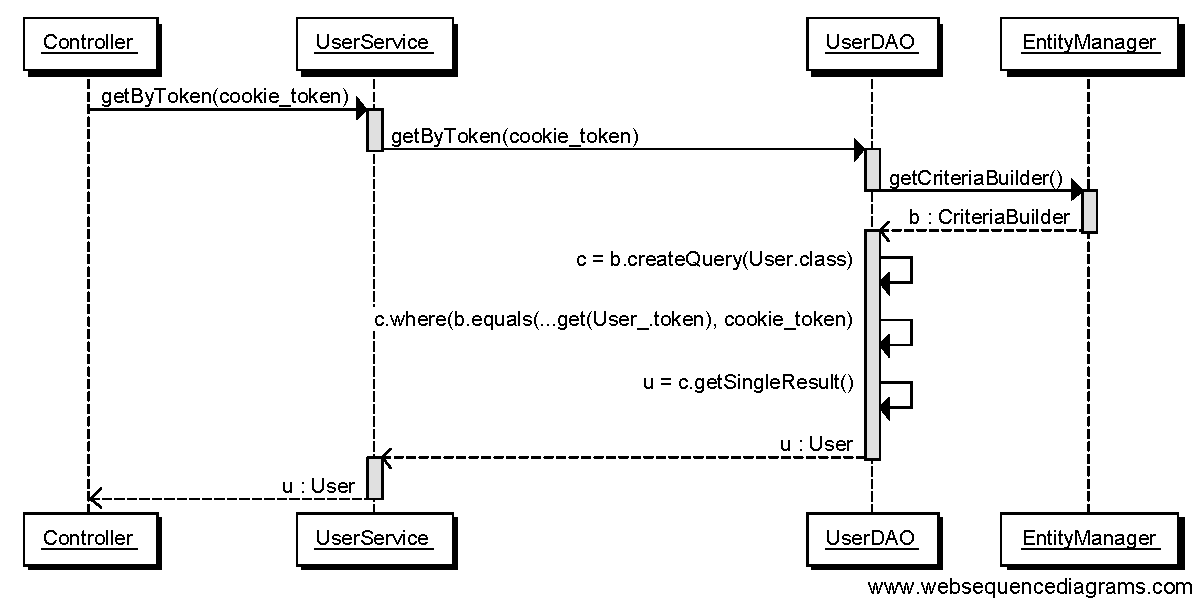
\includegraphics[width=\textwidth,trim=0 0.4cm 0
      0,clip]{fetch_user_sequence.pdf}
    \end{figure}
    \pagebreak
  \section{Record Ophalen}
    Sequence diagram gebruikt in de sequence diagrammen van sectie
    \ref{sec:get-record-sequence} tot en met \ref{sec:delete-record-sequence}.
    \begin{figure}[H]
      \label{fig:fetch-record-sequence}
      \centering
      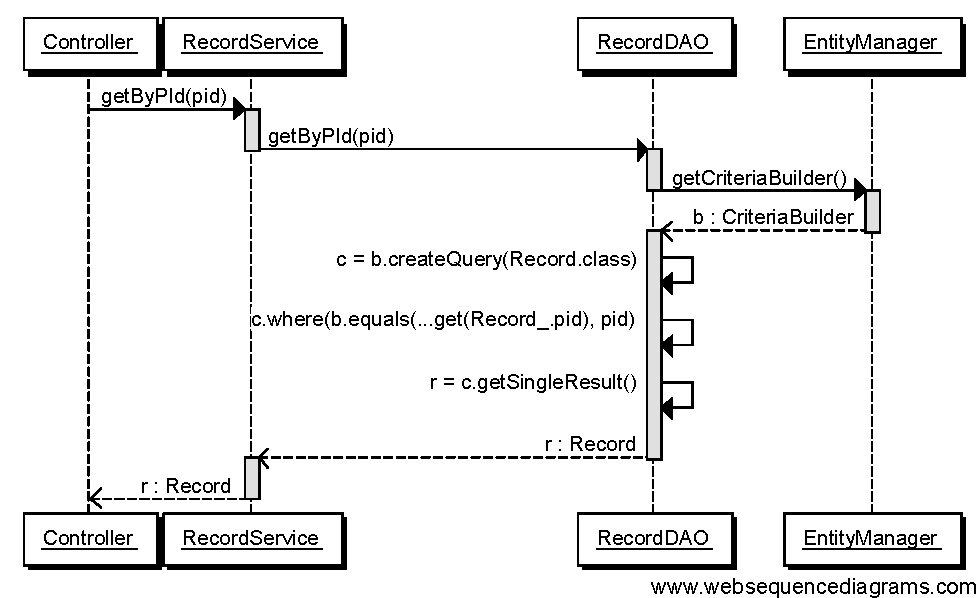
\includegraphics[width=\textwidth,trim=0 0.4cm 0
      0,clip]{fetch_record_sequence.pdf}
    \end{figure}
    \pagebreak

  \section{Specifieke Stukken Opvragen}
    \label{sec:get-record-sequence}
    \subsection{Gerelateerde API Specificaties}
      \begin{itemize}
        \item \textbf{\ref{ad:api:record:get:name}}
        \item \ref{ad:api:reservation:get:name}
        \item \ref{ad:api:permission:get:name}
      \end{itemize}
    \subsection{Sequence Diagram}
    \begin{figure}[H]
      \label{fig:get-record-sequence}
      \centering
      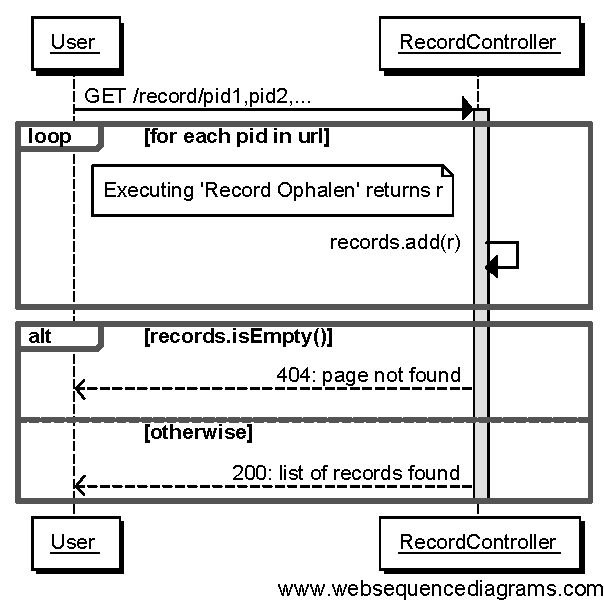
\includegraphics[width=0.6\textwidth,trim=0 0.4cm 0
      0,clip]{get_record_sequence.pdf}
    \end{figure}
    \pagebreak

  \section{Stukken Aanmaken/Wijzigen}
    \label{sec:put-record-sequence}
    \subsection{Gerelateerde API Specificaties}
      \begin{itemize}
        \item \textbf{\ref{ad:api:record:put:name}}
        \item \ref{ad:api:reservation:put:name}
        \item \ref{ad:api:permission:put:name}
      \end{itemize}
    \subsection{Sequence Diagram}
    \begin{figure}[H]
      \label{fig:put-record-sequence}
      \centering
      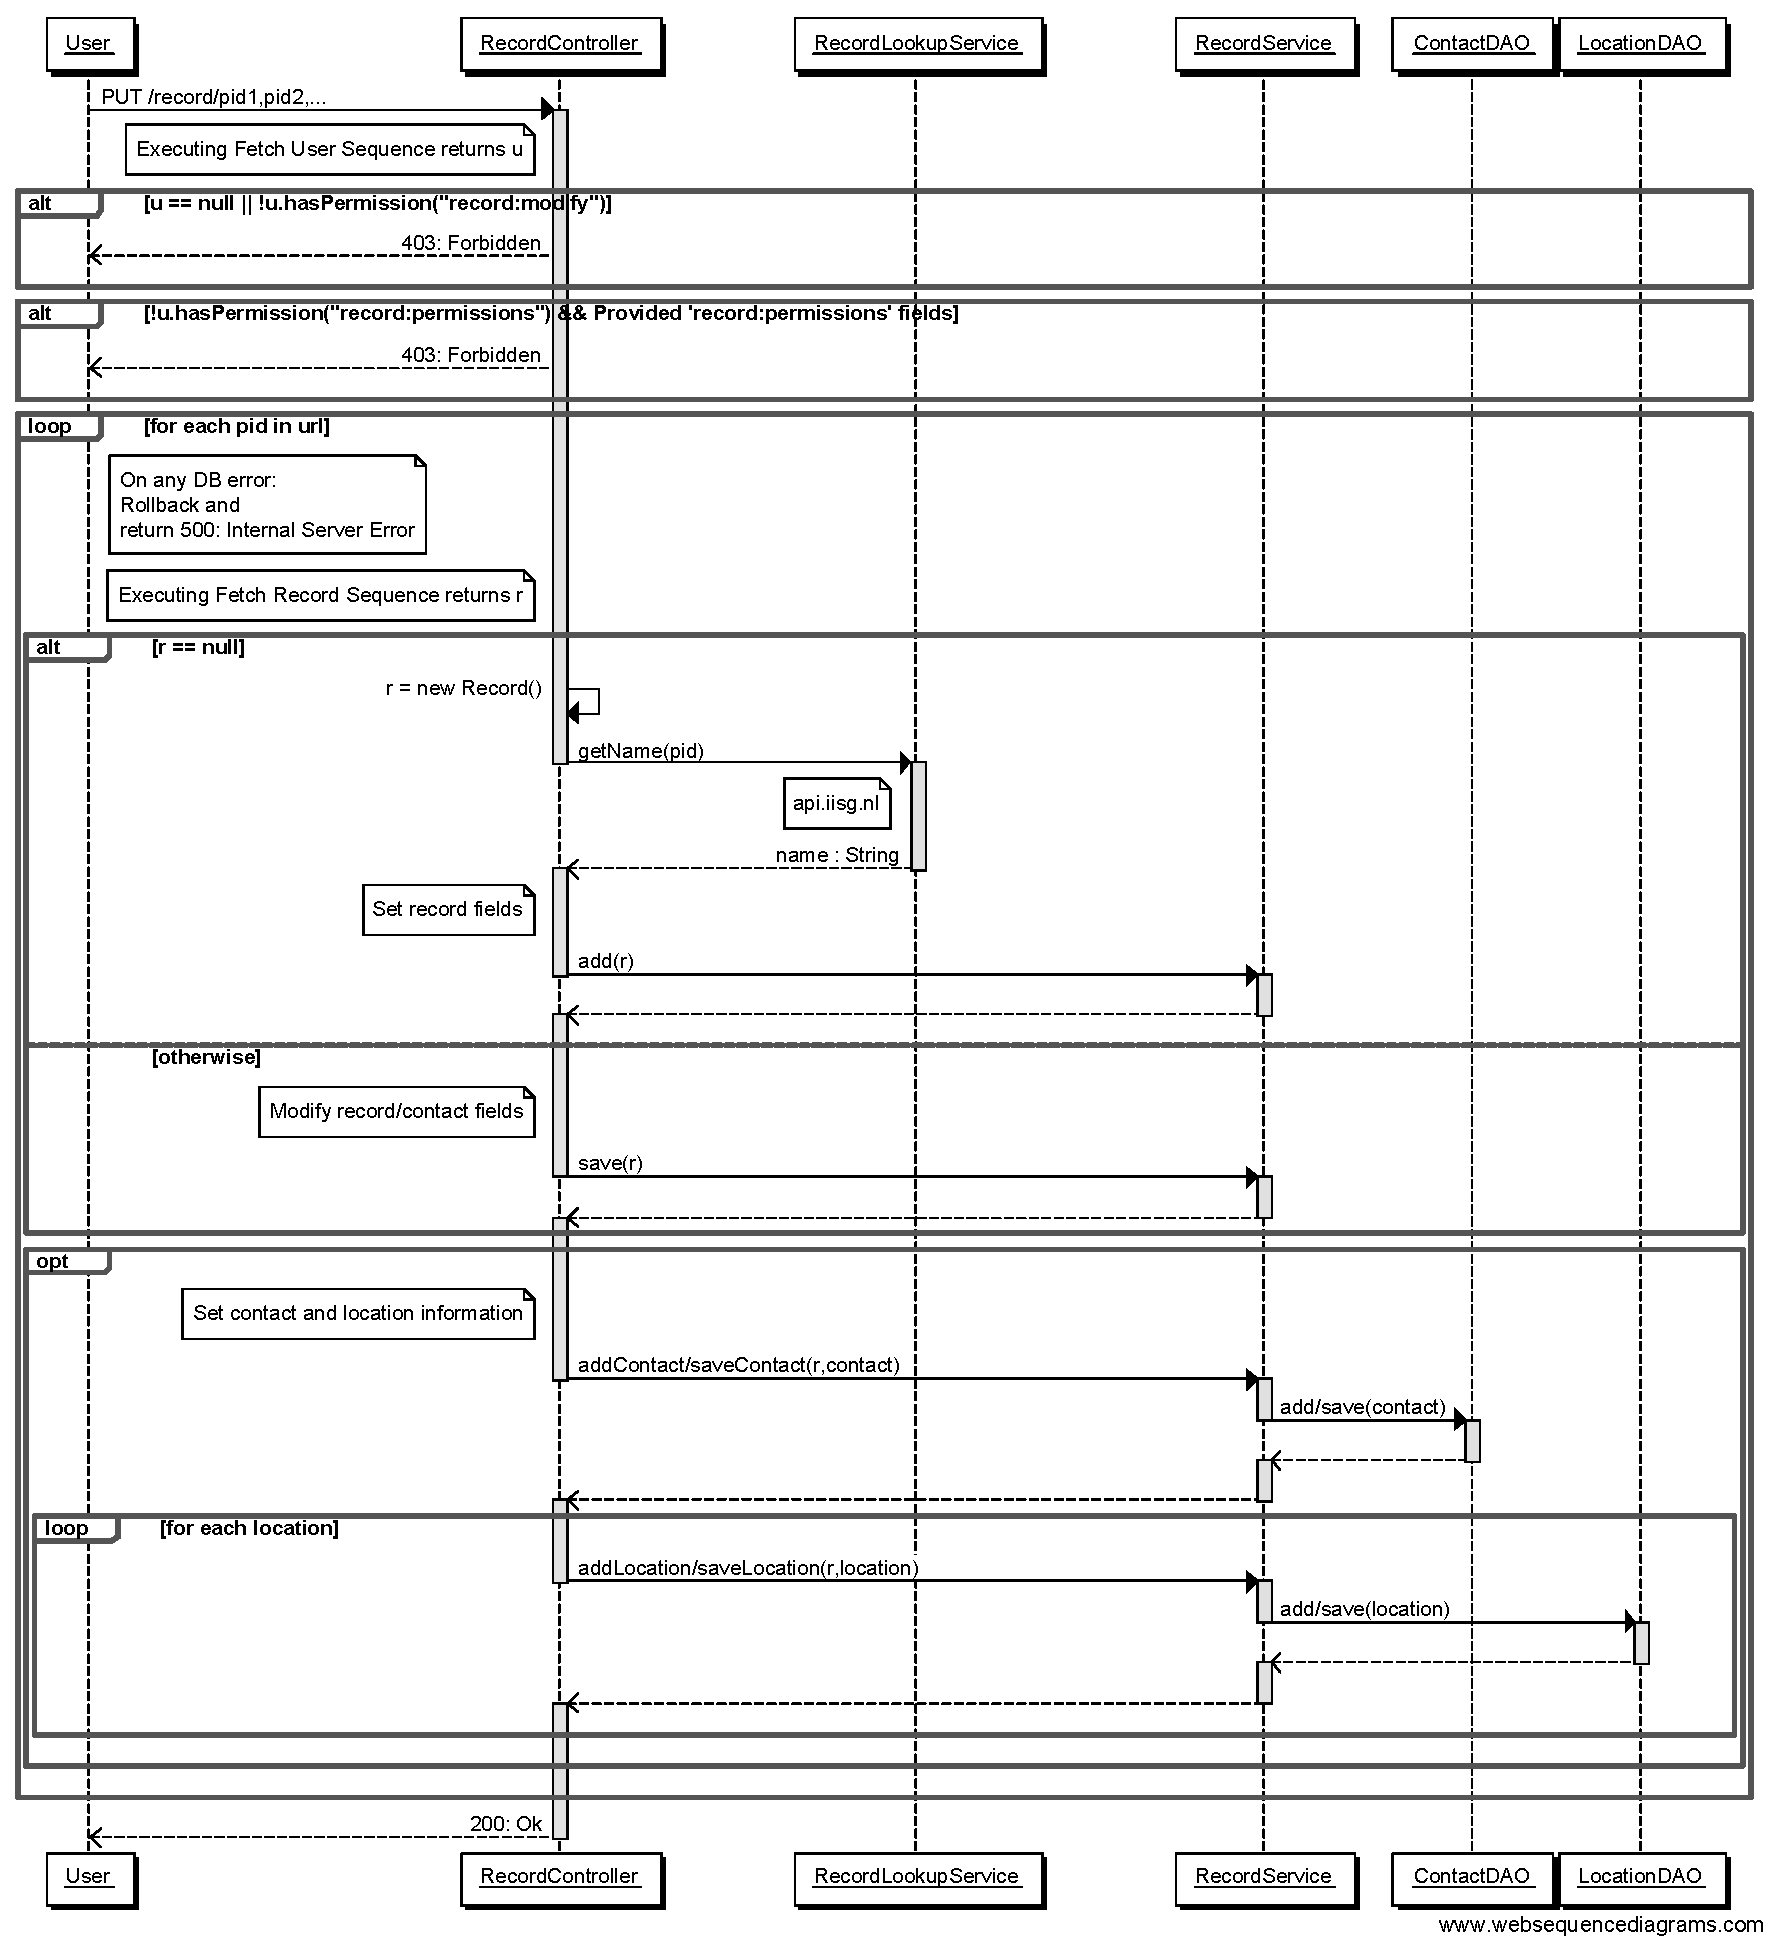
\includegraphics[width=\textwidth,trim=0 0.45cm 0
      0,clip]{put_record_sequence.pdf}
    \end{figure}
    \pagebreak

  \section{Stukken Verwijderen}
    \label{sec:delete-record-sequence}
    \subsection{Gerelateerde API Specificaties}
      \begin{itemize}
        \item \textbf{\ref{ad:api:record:delete:name}}
        \item \ref{ad:api:reservation:delete:name}
        \item \ref{ad:api:permission:delete:name}
      \end{itemize}
    \subsection{Sequence Diagram}
    \begin{figure}[H]
      \label{fig:delete-record-sequence}
      \centering
      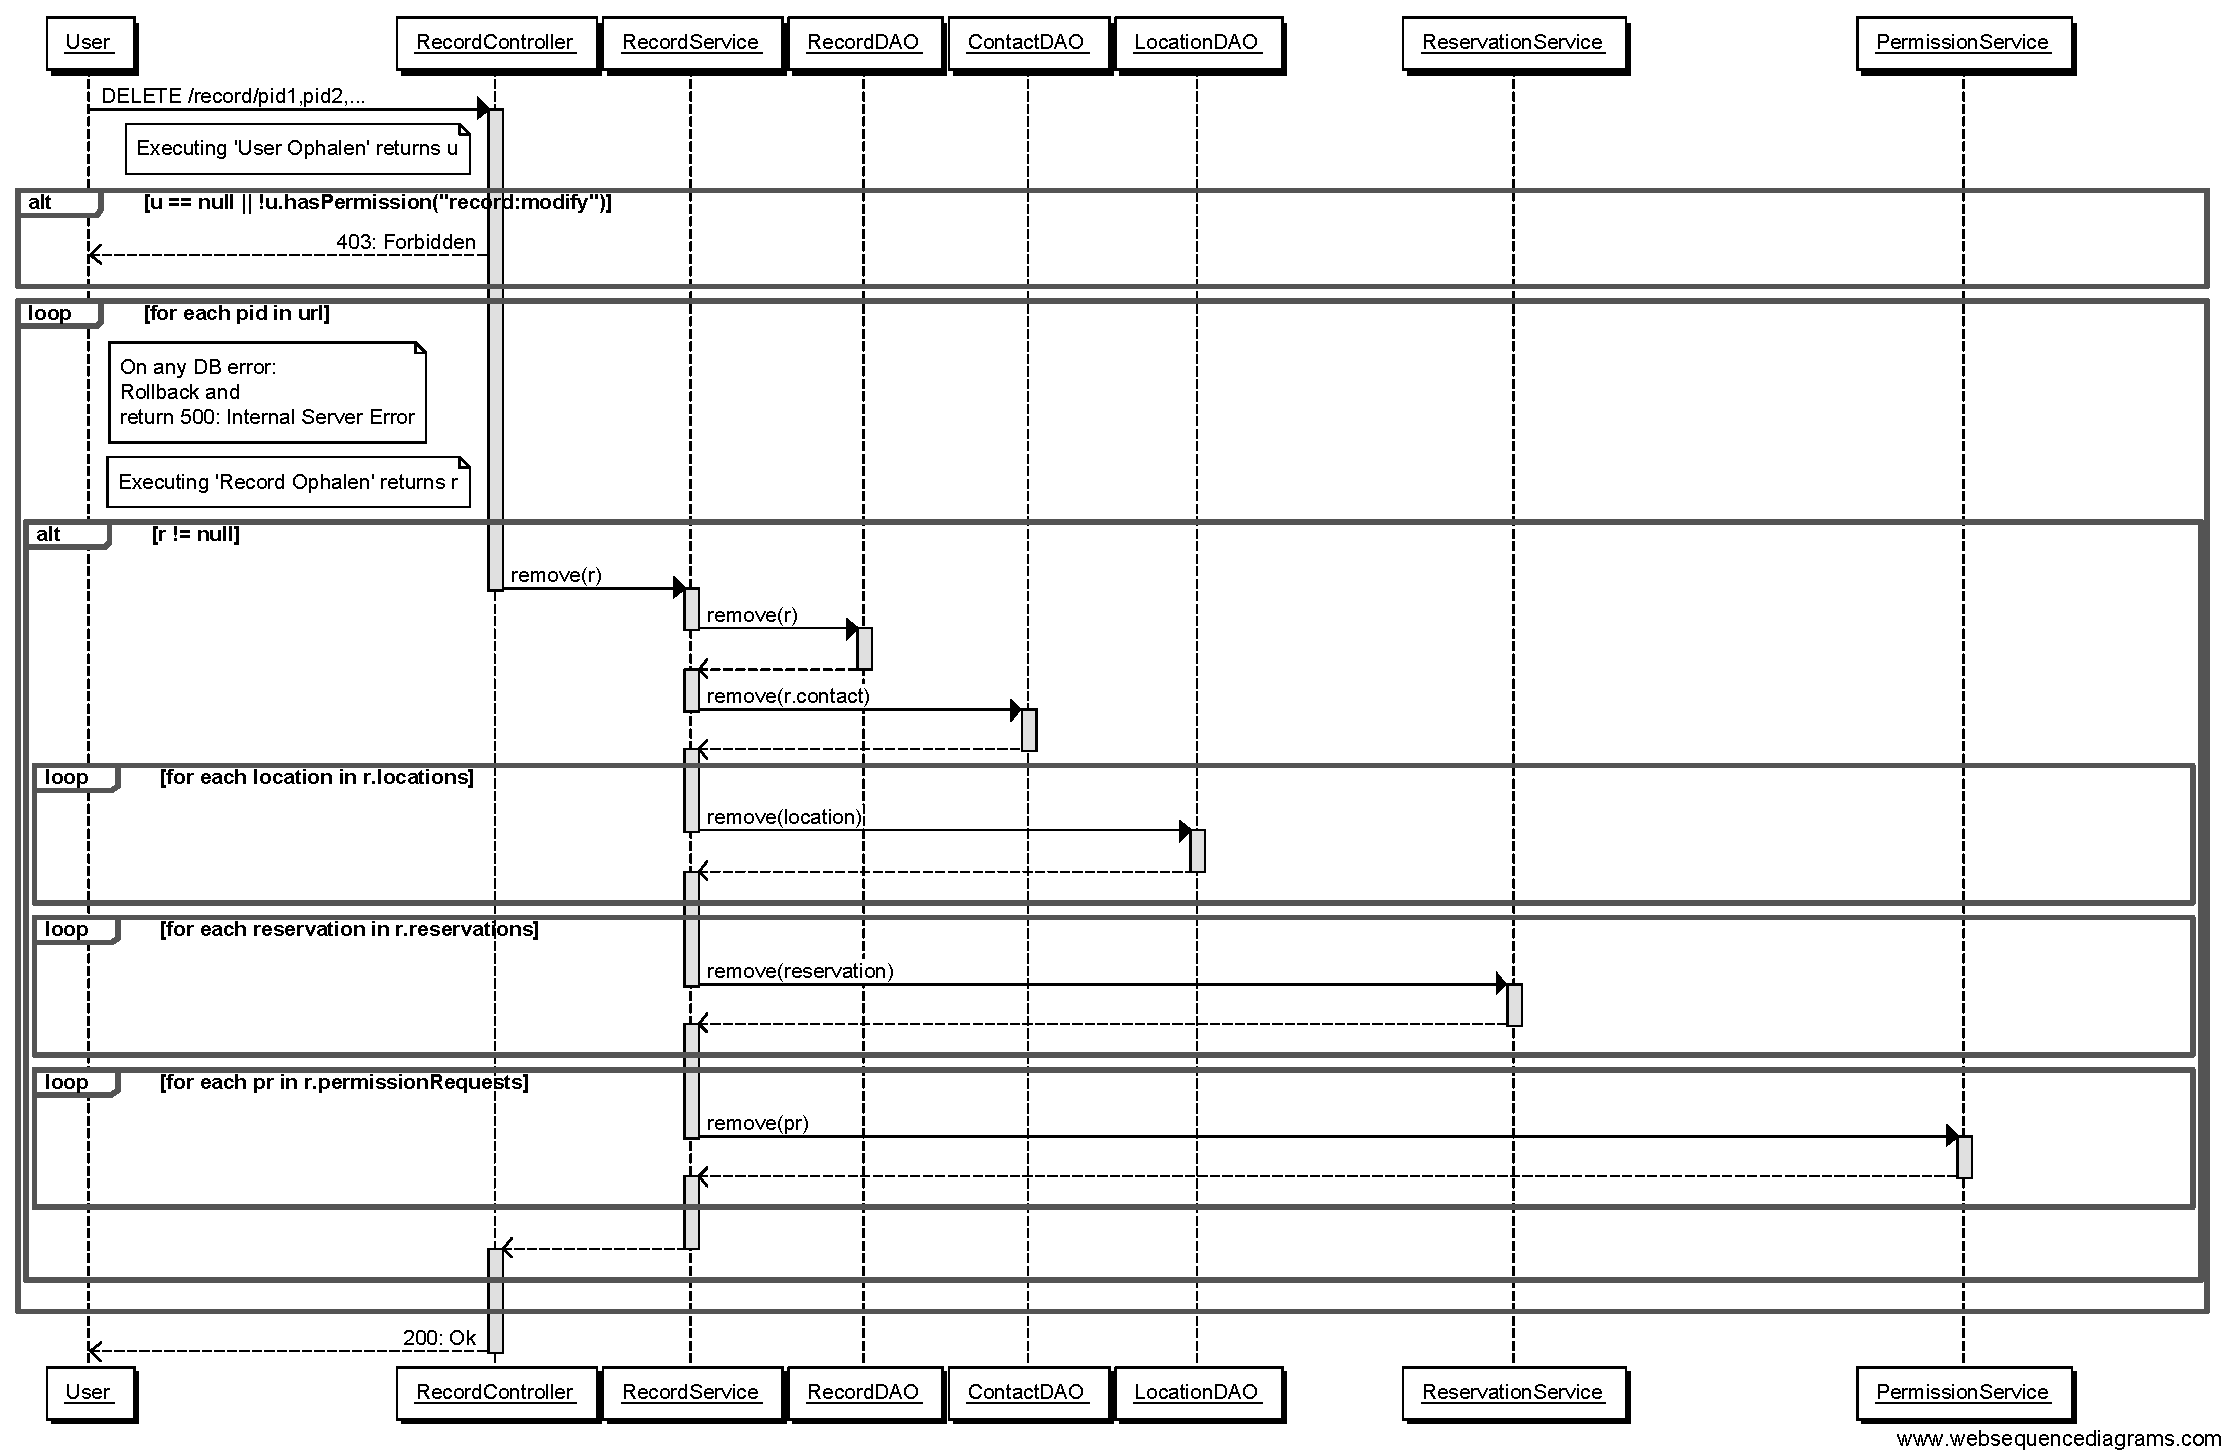
\includegraphics[totalheight=115mm,trim=0 0.4cm 0
      0,clip,angle=90]{delete_record_sequence.pdf}
    \end{figure}
    \pagebreak

  \section{Nieuwe Reservering Aanmaken}
    \subsection{Gerelateerde API Specificaties}
      \begin{itemize}
        \item \textbf{\ref{ad:api:reservation-list:post:name}}
        \item \ref{ad:api:permission-list:post:name}
      \end{itemize}
    \subsection{Sequence Diagram}
    \begin{figure}[H]
      \label{fig:post-reservation-sequence}
      \centering
      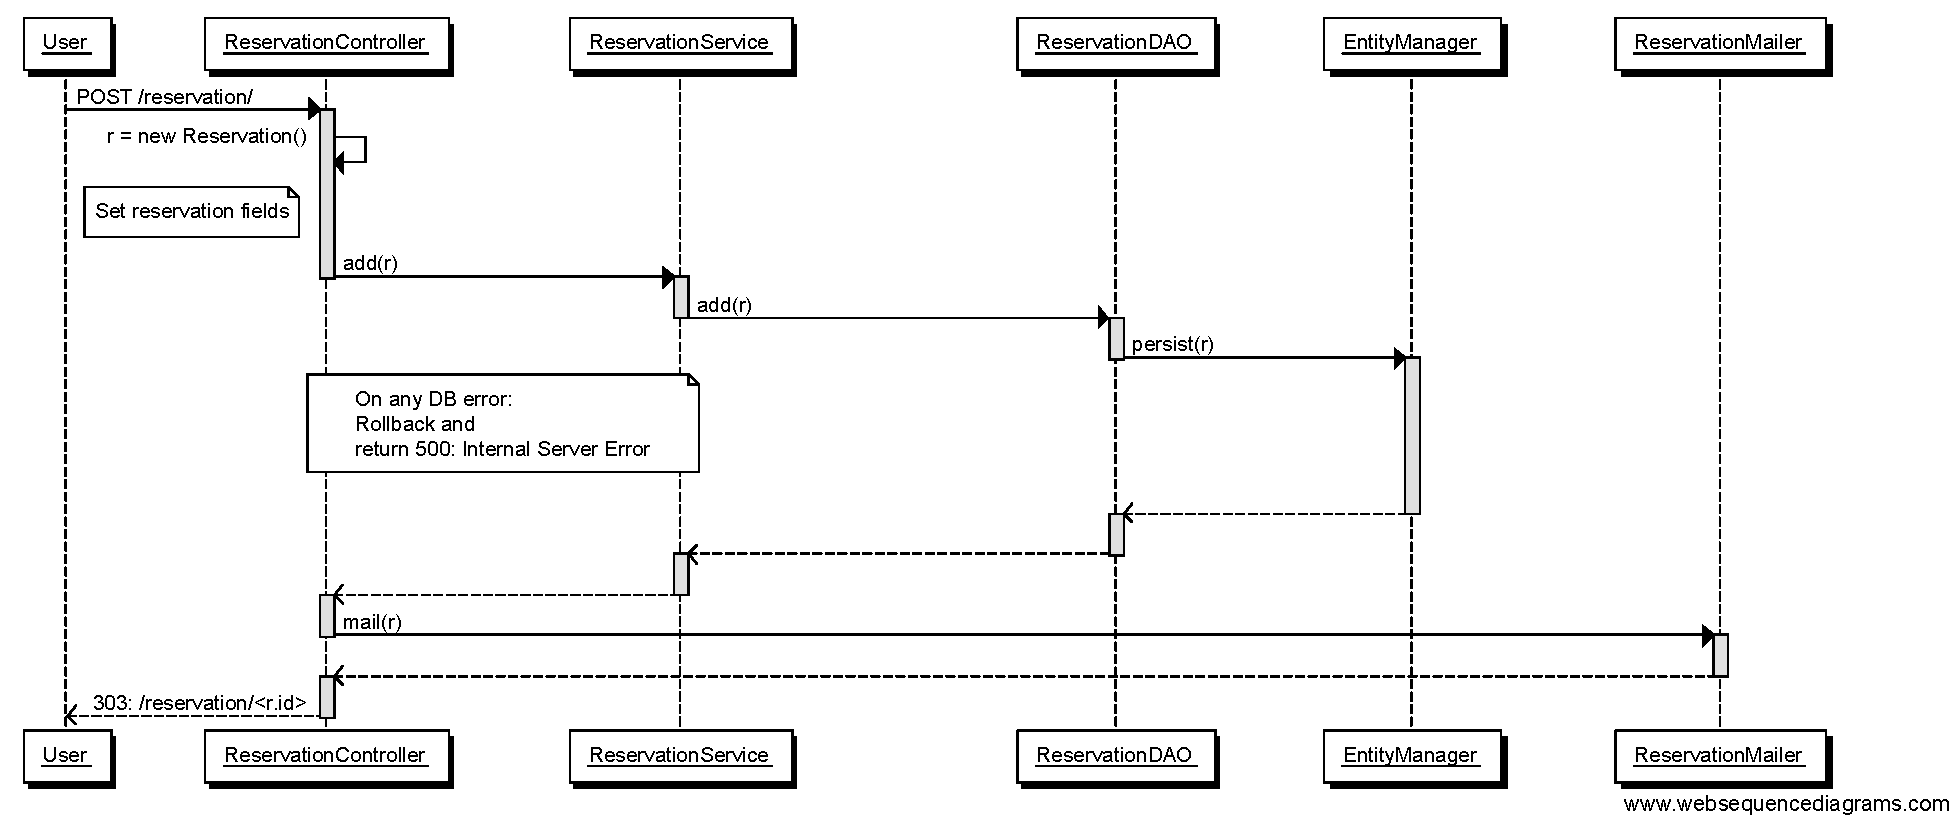
\includegraphics[width=\textwidth,trim=0 0.4cm 0
      0,clip]{post_reservation_sequence.pdf}
    \end{figure}
    \pagebreak

  \section{Lijst van Reserveringen Opvragen}
    \label{sec:get-records-sequence}
    \subsection{Gerelateerde API Specificaties}
      \begin{itemize}
        \item \textbf{\ref{ad:api:reservation-list:get:name}}
        \item \ref{ad:api:permission-list:get:name}
      \end{itemize}
    \subsection{Sequence Diagram}
    \begin{figure}[H]
      \label{fig:get-reservations-sequence}
      \centering
      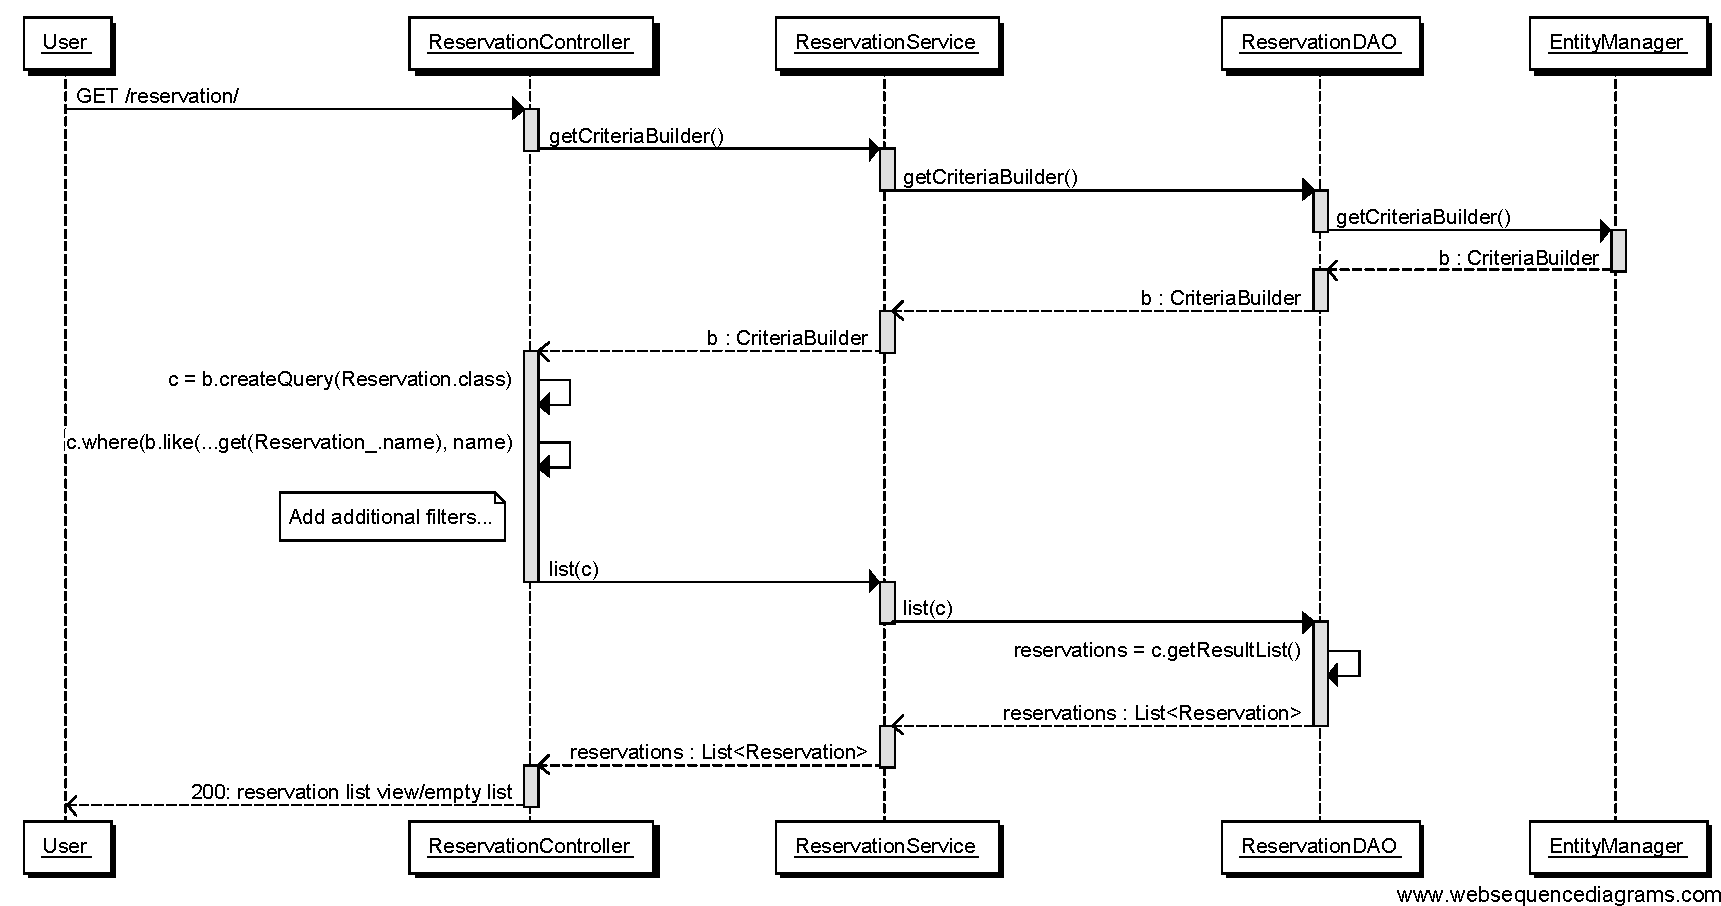
\includegraphics[width=\textwidth,trim=0 0.4cm 0 0,clip]{get_reservations_sequence.pdf}
    \end{figure}



\chapter{Hardware Omgeving}
\label{cha:hardware-omgeving}
Het systeem zal eerst in een test omgeving draaien voordat het, na
acceptatietests (zie bijlage \ref{cha:testplan}), naar productie
gaat. Er is daarom op hardware niveau onderscheid gemaakt tussen deze twee
omgevingen, zoals te zien is in figuur \ref{fig:hardware-omgeving}.

Binnen de testomgeving kan het uitprinten van reserveringen worden getest d.m.v.
een PDF-printer. Door middel van de SSH tunnel tussen de test en productieomgeving kan het
systeem in productie worden genomen.

    \begin{figure}[H]
      \centering
      \includegraphics[width=\textwidth,trim=0 0.4cm 0 0,clip]{hardware_mapping.pdf}
      \caption{Hardware omgeving}
      \label{fig:hardware-omgeving}
    \end{figure}

\printglossary[title=Verklarende Woordenlijst,toctitle=Verklarende Woordenlijst]
\appendix
\chapter{Implementatieplan}
  \label{cha:implementatieplan}
  De implementatie zal worden uitgevoerd in twee aparte iteraties. Bij de eerste
  iteratie zal het \gls{def:metadata}\glsadd{def:metadata} systeem worden opgezet en begonnen worden aan het
  aanmaken van aanvragen/reserveringen. Bij de tweede iteratie wordt de
  reserveringsfunctionaliteit afgemaakt en zou het mogelijk moeten worden om
  aanvragen voor toestemming in te vullen en te bemiddelen.

  Het bestellen van reproducties wordt niet bij de eerste milestone
  ge\"implementeerd omdat het benodigde systeem (de Shared Object Repository
  (\gls{def:sor}\glsadd{def:sor}))
  nog niet in gebruik is genomen, en er daarom geen werkend product zou kunnen
  worden afgeleverd.

  Voor beide iteraties volgt het \gls{def:moscow}\glsadd{def:moscow} schema met
  de eisen die worden ge\"implementeerd en de prioriteiten die gesteld zijn voor
  deze eisen.\\

  \begin{tabular}{| l l |}
    \hline
    \textbf{M} & Must have\\
    \textbf{S} & Should have\\
    \textbf{C} & Could have\\
    \textbf{W} & Won't have (but would like)\\
    \hline
  \end{tabular}\hfill

  \section{Iteratie 1}
    \hfill\\
    \begin{tabular}{| p{0.15\textwidth} p{0.15\textwidth} p{0.6\textwidth} |}
      \hline
      \textbf{Prioriteit} & \textbf{Timespan} & \textbf{Requirement} \\
      \hline
      M & Week 1 & \namedref{req:f:metadata}\\ \hline
      M & Week 1 & \namedref{req:f:status}\\ \hline
      M & Week 1 & \namedref{req:f:metadata-invullen}\\ \hline
      S & Week 2 & \namedref{req:f:aanvragen}\\ \hline
      S & Week 2 & \namedref{req:f:max-aantal-stukken}\\ \hline
      S & Week 2 & \namedref{req:f:voor-16-reserveren}\\ \hline
      S & Week 2 & \namedref{req:f:status-opvragen}\\ \hline
      C & Week 2 & \namedref{req:f:reserveringen-bekijken}\\ \hline
      C & Week 2 & \namedref{req:f:wachtnummertje}\\ \hline
      C & Week 2 & \namedref{req:f:print-vel}\\ \hline
    \end{tabular}

  \section{Iteratie 2}
    \hfill\\
    \begin{tabular}{| p{0.15\textwidth} p{0.15\textwidth} p{0.6\textwidth} |}
      \hline
      \textbf{Prioriteit} & \textbf{Timespan} & \textbf{Requirement} \\
      \hline
      M & Week 3 & \namedref{req:f:inloggen}\\ \hline
      M & Week 3 & \namedref{req:f:geenregistratie}\\ \hline
      M & Week 3 & \namedref{req:f:reserveringen-bekijken}\\ \hline
      M & Week 3 & \namedref{req:f:status-reservering}\\ \hline
      M & Week 3 & \namedref{req:f:status-opvragen}\\ \hline
      M & Week 3 & \namedref{req:f:aanvragen}\\ \hline
      M & Week 3 & \namedref{req:f:max-aantal-stukken}\\ \hline
      M & Week 3 & \namedref{req:f:voor-16-reserveren}\\ \hline
      S & Week 4 & \namedref{req:f:permissie}\\ \hline
      S & Week 4 & \namedref{req:f:wachtnummertje}\\ \hline
      S & Week 4 & \namedref{req:f:permissie-bemiddel}\\ \hline
      S & Week 4 & \namedref{req:f:print-vel}\\ \hline
      C & Week 4 & \namedref{req:f:auto-print}\\ \hline
      C & Week 4 & \namedref{req:f:permissie_bevestiging}\\ \hline
      W & Week 4 & \namedref{req:f:permissie_direct}\\ \hline
    \end{tabular}

\chapter{Testplan}
  \label{cha:testplan}
  \section{Test Methodiek}
    Om ervoor te zorgen dat het systeem naar behoren werkt, zal er op meerdere
    manieren worden getest. Voor elke iteratie zijn er verschillende test 
    categorie\"en:
    \begin{enumerate}
      \item \textbf{Unit Tests:} Binnen een klasse op methode niveau testen 
        van code. Dit zal worden gedaan bij alle niet-triviale methoden. Dit
        zorgt ervoor dat de werking van de methoden wordt gegarandeerd. Test
        specificaties worden \emph{ad-hoc} gespecificeerd waar nodig.
      \item \textbf{Integration Tests:} Dit type tests zorgt ervoor dat de samenwerking
        tussen klassen wordt getest. Voor zowel elk gespecificeerd sequence diagram
        uit hoofstuk \ref{cha:control-flow}, als voor alle soortgelijke control
        flows, zal er voor zover mogelijk een test worden geschreven. 
      \item \textbf{System Tests:} Dit type tests zorgt ervoor dat er aan de
        requirements wordt voldaan. Aan de hand van het test script in bijlage
        \ref{sec:testscript} zal worden gekeken of het systeem aan de opgestelde
        \glspl{def:fr}\glsadd{def:fr} voldoet. De \glspl{def:nfr}\glsadd{def:nfr}
        zullen worden beoordeeld in overleg met de projectleider.
      \item \textbf{Acceptance Tests:} Dit type tests zorgt ervoor dat het
        systeem ook daadwerkelijk doet wat de gebruiker ervan verwacht.
        Aangezien er een prototype wordt opgeleverd, zullen er geen acceptance
        tests worden uitgevoerd.
    \end{enumerate}


  \pagebreak
  \section{Test Script}
    \label{sec:testscript}
    Met dit test script wordt getest of het systeem aan de functionele
    requirements voldoet. Alvorens te beginnen met testen, dient de data uit
    bijlage \ref{sec:testdata} aanwezig te zijn in de database. In de tabel kan
    worden aangegeven dat een test geslaagd is (P van Pass), dat een test gefaald
    is (F van Failed) of dat een test niet uit te voeren is omdat er
    bijvoorbeeld op knoppen gedrukt moeten worden die nog niet zijn
    ge\"implementeerd (I van incomplete).

    \newcounter{step}
    \setcounter{step}{1}
    \makeatletter
      \def\c{\arabic{step}.\addtocounter{step}{1}}
    \makeatother
    \begin{longtable}{| m{0.05\textwidth} | m{0.38\textwidth}
      | m{0.38\textwidth} | m{0.08\textwidth} | m{0.07\textwidth} |}
      \hline
      & \textbf{Stap} & \textbf{Verwacht Resultaat} & \textbf{Getest}
      & \textbf{P/F/I} \\\hline
      \endhead

      \c &
      \par - Begin op de login pagina voor medewerkers.
      \par - Vul de gebruikersnaam ``Fout'' en het wachtwoord ``Fout'' in.
      \par - Klik op ``Login''.
      & Foutmelding dat het wachtwoord niet klopt of de gebruiker niet
      bestaat.
      & \ref{req:f:inloggen}
      & \\\hline

      \c &
      \par - Vul de gebruikersnaam ``Peter'' en het wachtwoord ``Fout'' in.
      \par - Klik op ``Login''.
      & Foutmelding dat het wachtwoord niet klopt of de gebruiker niet
      bestaat.
      & \ref{req:f:inloggen}
      & \\\hline

      \c &
      \par - Vul de gebruikersnaam ``Test'' en het wachtwoord ``Test'' in.
      \par - Klik op ``Login''.
      & De startpagina voor ingelogde medewerkers.
      & \ref{req:f:inloggen}
      & \\\hline
      \hline


      \c &
      \par - Klik op ``Bewerk Stukken''.
      \par - Vul in het `Zoek op titel' veld de naam ``Dora Russell'' in.
      \par - Klik op ``Zoek''.
      \par - Klik op het eerste archief in het resultaat.
      & \par - De PID en titel van het archief zijn zichtbaar.
        \par - Invulvelden voor metadata over het archief.
      & \ref{req:f:metadata-invullen}, \ref{req:f:metadata}
      & \\\hline

      \c &
      \par - Klik op de radiobutton ``Beperkt'' voor restrictie type.
      \par - Vul bij het tekstvak ``Restrictie Details'' de data ``Test Restrictie''
        in.
      \par - Klik op ``Opslaan''.
      & Een melding dat de gegevens succesvol zijn opgeslagen.
      & \ref{req:f:metadata-invullen}, \ref{req:f:metadata}
      & \\\hline

      \c &
      \par - Vul onder ``Locaties'' het type ``Microfilm'', verdieping
      ``4'' in, laat de overige velden leeg.
      \par - Klik op ``Locatie Toevoegen''.
      & Een melding dat de locatie is toegevoegd.
      & \ref{req:f:metadata-invullen}, \ref{req:f:metadata}
      & \\\hline

      \c &
      \par - Selecteer bij Gebruik Type de locatie ``Microfilm''.
      \par - Klik op ``Opslaan''.
      & Een melding dat de gegevens succesvol zijn opgeslagen.
      & \ref{req:f:metadata-invullen}, \ref{req:f:metadata}
      & \\\hline

      \c &
      \par - Klik op ``Bewerk Stukken''.
      \par - Vul de PID ``11051175\_MARC'' in.
      \par - Klik op ``Toon''.
      & \par - Invulvelden voor metadata over het archief.
        \par - Bestaande metadata van dit archief in de invulvelden.
        \par - De zojuist ingevulde restrictie voor het archief.
      & \ref{req:f:metadata-invullen}, \ref{req:f:metadata}
      & \\\hline

      \c &
      \par - Klik op ``Verwijder Metadata''.
      & \par - Een melding dat de record is verwijderd.
      & \ref{req:f:metadata-invullen}, \ref{req:f:metadata}
      & \\\hline

      \c &
      \par - Klik op ``Bewerk Stukken''.
      \par - Vul de PID ``11051175\_MARC'' in.
      \par - Klik op ``Toon''.
      & \par - Invulvelden voor metadata over het archief.
        \par - Geen ingevulde data in de velden.
      & \ref{req:f:metadata-invullen}, \ref{req:f:metadata}
      & \\\hline
      \hline

      \c &
      \par - Klik op ``Reserveringsoverzicht''.
      & \par De aanvraag in de database.
      & \ref{req:f:reserveringen-bekijken}
      & \\\hline

      \c &
      \par - Selecteer de aanvraag en klik op ``Print Locaties''.
      & \par 4 printjes: 2 voor elk stuk in de aanvraag.
      & \ref{req:f:reserveringen-bekijken}, \ref{req:f:print-vel}
      & \\\hline

      \c &
      \par - Klik op ``Scan Items''.
      \par - Vul een item nummer uit de print in (staat onder de barcode) in en
      druk op Enter (scan indien mogelijk de print).
      \par - \emph{Herhaal deze stap voor het andere item uit de reservering.}
      & \par - De reservering is naar status ``Actief'' veranderd.
        \par - Het ingevoerde item is van status ``Aangevraagd'' naar status
        ``Uitgeleend'' veranderd.
      & \ref{req:f:status}, \ref{req:f:status-reservering}
      & \\\hline

      \c &
      \par - Vul een item nummer uit de print in (staat onder de barcode) in en
      druk op Enter (scan indien mogelijk de print).
      \par - \emph{Herhaal deze stap voor het andere item uit de reservering.}
      & \par - Het ingevoerde item is van status ``Uitgeleend'' naar status
        ``Teruggebracht'' veranderd.
      & \ref{req:f:status}, \ref{req:f:status-reservering}
      & \\\hline

      \c &
      \par - Vul een item nummer uit de print in (staat onder de barcode) in en
      druk op Enter (scan indien mogelijk de print).
      \par - \emph{Herhaal deze stap voor het andere item uit de reservering.}
      & \par - Het ingevoerde item is van status ``Teruggebracht'' naar status
        ``Beschikbaar'' veranderd.
        \par - Indien dit het laatste item uit de reservering was is de status
        van de reservering naar ``Afgehandeld'' veranderd.
      & \ref{req:f:status}, \ref{req:f:status-reservering}
      & \\\hline
      \hline

      \c &
      \par - Klik op ``Toestemmingsaanvragen''.
      & \par De toestemmingsaanvraag die in de database staat.
      & \ref{req:f:permissie-bemiddel}
      & \\\hline

      \c &
      \par - Klik op de weergegeven toestemmingsaanvraag.
      & \par De twee stukken die zijn aangevraagd: 15 en 16 van het archief
      ``Alexander Berkman Papers''.
      & \ref{req:f:permissie-bemiddel}
      & \\\hline

      \c &
      \par - Klik bij item 15 op ``Toestemming Geven'' en bij item 16 op
      ``Toestemming Weigeren''.
      \par - Klik ``Opslaan''.
      & \par De toestemmingsaanvraag is gemarkeerd als afgehandeld.
      & \ref{req:f:permissie-bemiddel}
      & \\\hline
      \hline


      \c &
      \par - Ga naar de interface voor bezoekers.
      \par - Ga naar de pagina om een aanvraag te maken voor item 13 en 14 in
      ``Alexander Berkman Papers''.
      & \par Invulvelden voor naam, email en datum.
      & \ref{req:f:aanvragen}
      & \\\hline

      \c &
      \par - Vul de naam ``Test Test'' en het email ``test.test@example.com''
        in.
      \par - Vul de huidige datum in.
      \par - Klik op ``Reserveer''.
      & \par - Een bericht dat de aanvraag met succes is opgeslagen.
        \par - Een willekeurig wachtnummer voor de reservering.
        \par - Indien het automatisch printen is ge\"implementeerd, een uitdraai
        van de gereserveerde stukken.
      & \ref{req:f:aanvragen}, \ref{req:f:auto-print}
      & \\\hline

      \c &
      \par - Ga naar de interface voor bezoekers.
      \par - Ga naar de pagina om een aanvraag te maken voor item 14 in
      ``Alexander Berkman Papers''.
      & \par Melding dat het stuk niet beschikbaar is.
      & \ref{req:f:aanvragen}
      & \\\hline

      \c &
      \par - Ga naar de interface voor bezoekers.
      \par - Ga naar de pagina om een aanvraag te maken voor item 15 in
        ``Alexander Berkman Papers''.
      & \par De melding dat het archief restricties heeft en de vraag of 
        er een aanvraag voor toestemming moet worden gemaakt.
      & \ref{req:f:permissie}
      & \\\hline

      \c &
      \par - Klik op ``Vraag Toestemming Aan''.
      \par - Vul in naam ``John Doe'' en email ``test.test@example.com''.
        Vul bij huidig onderzoek de waarde ``Test Script'' in.
      \par - Klik op ``Aanvragen''.
      & \par Een bericht dat de aanvraag voor toestemming met succes is
        opgeslagen en er een e-mail wordt verstuurd zodra deze is afgehandeld.
      & \ref{req:f:permissie}
      & \\\hline
    \end{longtable}

  \pagebreak
  \section{Test Data}
    \label{sec:testdata}
    De test database moet bestaan uit de volgende data om het test script te
    kunnen voltooien:

    \subsection{Gebruikers}
      \begin{enumerate}
        \item ``Test'' met wachtwoord ``Test''. Volledige privileges.
        \item ``Fout'' met wachtwoord ``Test''. Geen privileges.
      \end{enumerate}
    \subsection{Archieven}
      \begin{enumerate}
        \item Een archief met de naam ``Alexander Berkman Papers'' en PID
        ``10729085\_EAD''.
      \end{enumerate}
    \subsection{Records}
      \begin{enumerate}
        \item Een record met inventarisnummer 13 voor het archief ``Alexander Berkman Papers'' met de
        restrictie Open, geen contactinformatie, geen embargo en de locatie
        velden volledig ingevuld (microfilm/origineel). Het gebruik type is
        gezet op ``Microfilm''
        \item Een record met inventarisnummer 14 voor het archief ``Alexander Berkman Papers'' met de
        restrictie Open, geen contactinformatie, geen embargo en de locatie van
        het origineel slechts ``Verdieping 4''.
        \item Een record met inventarisnummer 15 voor het archief ``Alexander Berkman Papers'' met de
        restrictie Beperkt, contactinformatie, geen embargo en de locatie
        slechts ``Verdieping 5''.
        \item Een record met inventarisnummer 16 voor het archief ``Alexander Berkman Papers'' met de
        restrictie Beperkt, contactinformatie, geen embargo en de locatie
        slechts ``Verdieping 5''.
      \end{enumerate}
    \subsection{Aanvragen}
      \begin{enumerate}
        \item Een aanvraag voor items 13 en 14 in ``Alexander Berkman Papers'' met
          naam ``John Doe'' en email ``john.doe@iisg.nl'', status
          ``Aangevraagd''.
      \end{enumerate}
    \subsection{Aanvragen voor Toestemming}
      \begin{enumerate}
        \item Een aanvraag voor toestemming op naam ``Test Test'' en email
        ``test.test@example.com'' voor item 15 en 16 van het archief
        ``Alexander Berkman Papers''.
      \end{enumerate}

\end{document}
